\chapter{VMT}
\section{Descripción general}
VMT es una herramienta para la edición y posterior ejecución de un espectáculo de video mapping, el que puede utilizar uno o más proyectores eventualmente alejados físicamente unos de otros para obtener un mejor cubrimiento de la escena a mapear. Para dar soporte al escenario distribuido, se cuenta con componentes remotos (cliente) con el fin de reproducir los efectos y eventos existentes del espectáculo. Mediante un editor tridimensional, es posible observar de forma centralizado lo que se ha producido hasta el momento así como visualizar la salida de cada uno de los proyectores a modo de validación. Si bien es un editor tridimensional se manejan conceptos bidimensionales de capa (layer) y cuadrante (quad), los que se pueden agregar y asociar a una cámara o proyector sin un limite predeterminado. Se proveen de mecanismos de calibración separadamente para objetos tridimensionales y bidimensionales utilizados al trabajar sobre la escena real luego de un primer escaneo. Dichos mecanismos serán explicados en detalles más adelante.

Las alternativas en cuanto a efectos de mapeo son de degrades (fade) de colores y la aplicación de texturas de imagen o video. Se cuenta también con un efecto para la animación de la posición de los objetos en tiempo de ejecución del espectáculo. Es posible visualizar en todo momento la ejecución de los efectos y su correspondiente impacto en la escena, y estos pueden ser lanzados por tiempo, por eventos de teclado o MIDI. Existe una linea de tiempo navegable, permitiéndose avanzar o retroceder a un intervalo de tiempo dado en el que queremos concentrarnos durante la producción del evento. Se permite agregar una única pista de audio en sincronía con el tiempo transcurrido del evento.

La interfaz gráfica de usuario está basada enteramente en botoneras y ventanas de propiedades flotantes para poder tener una vista mejorada y en tiempo real de lo que está sucediendo en la escena. Se proveen mecanismos para almacenar y cargar en archivos XML estándar toda la definición de la escena.

La tecnología de base seleccionada para la creación de los módulos de nuestra herramienta y todas las bibliotecas de terceros que se han utilizado son multiplataforma, lo que permite la compilación y ejecución en los entornos mas utilizadas hoy en día como Microsoft Windows, Linux y Mac OS.

\section{Descripción de módulos}

\subsection{Motor gráfico}
Para dar soporte a la visualización de elementos gráficos bidimensionales y tridimensionales en pantalla o proyectados y, el correspondiente mapeo de texturas de imágenes o videos sobre ellos tanto en la aplicación cliente como en la del editor del servidor, se creo un componente reusable para el motor de dibujado llamado \emph{vmt\_engine}. Este motor gráfico ofrece una interfaz programática genérica para el manejo y edición de objetos y efectos que contiene.

Los elementos bidimensionales son cuadriláteros y en la aplicación se llaman quads. Los quads se definen mediante las coordenadas bidimensionales en el plano de la imagen de los cuatro vértices que los componen. Se pueden posicionar en la pantalla de forma tal que al ser proyectados cubran una superficie total o parcial. Luego, sobre estos quads se aplicarán texturas en forma de imagen o video, para que la proyección deforme estas texturas adaptándolas a la forma del quad.
Los quads también pueden ser utilizados como máscaras para cubrir zonas de otros quads o elementos tridimensionales. Una máscara es básicamente un quad opaco de color negro. Dado que el color negro es el menos visible al ser proyectado, es útil para bloquear secciones que, por la geometría de la escena, podrían estar quedando mal proyectadas o iluminando zonas indeseadas.

En cuanto a los elementos tridimensionales, estos representan objetos más complejos y ofrecen una mayor versatilidad para realizar mapeos sobre ellos.
Estos objetos se cargan a partir de modelos tridimensionales en el formato estándar 3DS[The Labs: 3DS File Format, by Jeff Lewis - www.the-labs.com/Blender/3dsspec.html] y se permite cargar al motor cualquier geometría que lo respete.
La edición de la geometría de estos objetos es en general un tema complejo pero bien resuelto por varias aplicaciones de edición 3D como pueden ser 3DS Max[usa.autodesk.com/3ds-max] y Blender[www.blender.org] entre otros. Por esta y otras razones es que se delega la edición de las formas tridimensionales a programas para este propósito.
Los programas de edición además de permitir modificar la geometría manipulando vértices y caras, también posibilitan la definición de materiales para aplicar propiedades comunes a una cierta selección de caras de la malla 3D [glosario]. VMT utiliza estas selecciones de caras para mapear texturas sobre ellas resolviendo de esta forma el mapeo en tres dimensiones.

El mapeo tridimensional se realiza básicamente definiendo las coordenadas de mapeo en cada vértice del modelo 3DS. Las aplicaciones de edición 3D antes mencionadas proveen herramientas para hacer esta tarea de forma muy intuitiva. Ejemplo de esto es la definición de coordenadas de mapeo de un cilindro para mapear una textura en una columna cilíndrica.
Los elementos gráficos por sí mismos no son representables. Es necesario asignarles primero un material dentro de VMT y es a este material que se le asigna un color o una textura con la cual se representará el objeto.
En la implementación de los materiales se utilizan shaders [glosario], que son programas que se ejecutan en los procesadores gráficos y tienen como ventaja que son altamente paralelizables, permitiendo realizar cálculos de forma más rápida y eficiente. En la aplicación se utiliza el lenguaje de shaders para OpenGL GLSL ([www.lighthouse3d.com/opengl/glsl]) para la implementación de un shader básico que combina una textura de imagen o video con un color para obtener el resultado visibles del material. Este color tiene un canal alfa\footnote(Ver glosario.) y por lo tanto se pueden lograr texturas y colores con niveles de transparencia. No se esta considerando la iluminación en nuestra implementación del shader.

Para visualizar los elementos tridimensionales es necesario definir un punto de vista. Esto se logra mediante el agregado de una cámara en el motor y la configruación de sus propiedades, entre ellas su ubicación o punto de vista. Los proyectores con los que se realiza el espectáculo de video mapping son también representados como cámaras en el motor, pero no toda cámara configurada representa un proyector, ya que se pueden contar con cámaras que representen puntos de vista de un observador del espectáculo que sea de interés para el creador.
Las cámaras permiten ajustar sus parámetros mediante operaciones comunes a cámaras virtuales de forma similar a lo que ocurre en otros paquetes de animación por software y a cámaras cinematográficas en general. Estas operaciones representan movimientos de la cámara llamados Roll, Orbit, Dolly y Pan. Roll se refiere al movimiento en donde la posición de la cámara y el punto de vista son fijos y ésta rota a través del eje formado por ellos. Orbit es cuando la cámara orbita alrededor de su punto de vista, es decir, la posición de la cámara cambia pero siempre visualizando el mismo punto y manteniendo la distancia a este. Dolly es el movimiento en donde se mantienen el punto y la dirección de vista pero se mueve la posición de la cámara acercándose y alejándose del objetivo. Por último, Pan es el tipo de movimiento en el que cuando se mueve la cámara cambiando la posición y el punto de vista, se mantiene un paralelismo con la dirección.

\begin{figure}[H]
  \centering
    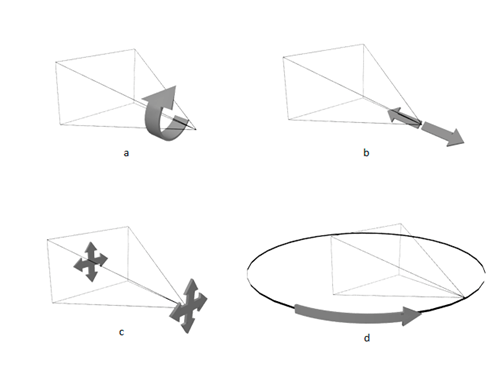
\includegraphics[width=0.5\textwidth]{./Cap5_vmt/vmtengine-cameramove.png}
  \caption{Movimientos de cámara. a) Roll b) Dolly c) Pan d) Orbit}
  \label{fig:VMT-CameraMove}
\end{figure}

Aparte de estos parámetros de ubicación, también existe el parámetro FOV (Field Of View) o campo de vista que es el ángulo de apertura de la cámara. Para el caso de cámaras que representan proyectores, este parámetro debe coincidir con el FOV del proyector para ajustar correctamente las escenas con respecto a lo que muestra la cámara en pantalla.
Mediante estas operaciones es que las cámaras virtuales de VMT ajustan sus parámetros para que la proyección de objetos tridimensionales coincida con las superficies proyectadas.
Hay que destacar que las cámaras proveen un punto de vista solo para los elementos tridimensionales. Los quads, que como se menciono son contrucciones bidimensionales, no dependen del punto de vista de la cámara y se representan en un sector de la pantalla relativo a esta. Es por esto que los quads no alteran su posición en pantalla al ajustar los parámetros de la cámara.

Los quads se pueden organizar en grupos de quads y pertenecen a una o mas capas, y cada capa pertenece a una única cámara de manera de representar las zonas a cubrir por un solo proyector. A su vez se permite aplicar una transformacion inicial a una capa, la que se aplicara a todos los quads o grupos de quads contenidos en ella. Esto es útil para ajustar la proyección de los quads en caso de mover el proyector levemente y que esta proyección deje de coincidir con las superficies, y provee la funcionalidad basica y de bajo nivel para el mecanismo de calibracion bidimensional que se detallara mas adelante.

Las texturas se asocian a grupos de quads solamente. Los grupos también permiten variar de forma limitada como se mapean las texturas a los quads que lo componen. Pueden ser mapeadas por cara en donde a cada uno de los quads se le mapeará toda la textura, o también de forma “plana”. Esto último significa que la textura será mapeada al conjunto entero de quads como si estos fueran trozos de un quad de mayor tamaño compuesto por todos ellos.

\begin{figure}[H]
  \centering
    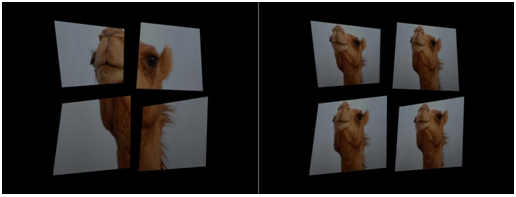
\includegraphics[width=0.5\textwidth]{./Cap5_vmt/vmtengine-maping.png}
  \caption{Izquierda: Proyección plana. Derecha: Proyección por cara.}
  \label{fig:VMT-Projection}
\end{figure}

Con estas variantes de proyección se le dan más posibilidades a un artista para lograr los efectos utilizados normalmente en espectáculos de video mapping.

El motor gráfico también contiene los efectos que se ejecutarán durante el espectáculo. Se aceptan como efectos la asignación de texturas en forma de imagen o video, ya sea a grupos de quads u objetos tridimensionales, el degrade de colores o fade en un material desde un color inicial a otro final, y la animación de la posición de un objeto tridimensional de un origen a un destino en un lapso de tiempo dado.

El efecto de mapeo de texturas es el más básico pero también el más potente en cuanto a la gran cantidad de alternativas al momento de mapear texturas sobre superficies. La variedad y la complejidad de las texturas está en la creación de los recursos de imagen o video que se deseen mapear. Al permitirse mapear estas texturas sobre objetos tridimensionales no es necesario distorsionar la forma de los videos sino que será el motor quien los adaptará a la forma del objeto que está siendo mapeado. El efecto de fade puede ser combinado en un objeto que ya disponga de una textura y así permitir por ejemplo su atenuación o resaltado. La duración del fade, al igual que la de animación de posición, es configurable.

Cabe aclarar que el estado final de la escena y todos los objetos contenidos en ella sera el que resulte luego de la finalización de los efectos. Esto es, si un objeto es de color rojo, y tiene un efecto de fade al azul aplicado, su color luego de la ejecución del efecto continuará siendo azul.

Un punto posible de extensión en el motor es la creación de más efectos genéricos como pueden ser animación de rotación, escala o modificadores de objetos tridimensionales, para dar mas posibilidades al usuario al momento de la creación del espectáculo.

Como se mencionó anteriormente, una de las tareas principales del motor gráfico es la representación en pantalla o la proyección de los elementos gráficos. La implementación del dibujado en si se realiza en un bucle principal de la aplicación encargado de actualizar todos los objetos de la escena de ser necesario, procesar los eventos pendientes y finalmente dibujar el resultado. Esto es un proceso cíclico que se repite varias veces por segundo.
En cada uno de estos ciclos se generan los frames que son las imágenes que se muestran como resultado final.
Para dar la ilusión de continuidad, la frecuencia de estos ciclos debe ser alta. En el caso de \emph{vmt\_engine} ésta se predetermina en 60 ciclos por segundo aunque alcanzar ésta frecuencia dependerá de varios factores como cantidad de quads, tamaño de texturas utilizadas, capacidad de procesamiento y memoria de los equipos.
Si esta frecuencia se encuentra muy por debajo de los 60 ciclos, la reproducción del espectáculo no será fluida y se podrían percibir saltos o pausas al reproducirlo.
Para que esta frecuencia efectivamente se logre es necesario que el procesamiento de cada uno de los ciclos del bucle principal sea eficiente. Esta eficiencia se logra reduciendo el costo de procesamiento en cada tareas u operación. A continuación se muestra un pseudo-código del bucle principal de dibujado y se analizan cada una de las acciones que se toman, su impacto en cuanto al rendimiento del programa y las medidas que se tomaron para su optimización:

Posicionar cámara
para todo objeto3d en la escena:
   para toda selección de caras:
       cargar material
       dibujar caras con el material
   fin
fin
Reset cámara
para todo quad
   cargar material
   dibujar quad
fin

Un bucle de este estilo cuenta con varios cuellos de botella.
La carga de materiales implica copiar una textura a la zona de la memoria de video correspondiente para utilizarla. Esto podría ser un proceso lento si no se disponen las texturas precargadas en memoria. Es por esta razón es que las texturas se cargan desde un comienzo en memoria y luego se utilizan referencias para identificarlas y asociarlas a una unidad de textura de OpenGL [www.opengl.org/wiki/Texture] para finalmente poder utilizarla.
Otra optimización pasa por hacer uso de shaders para el cálculo del resultado visual final.
La visualización fluida de un espectáculo de video mapping es difícil de predecir ya que, como se puede ver en el pseudo-codigo, los tiempos de ejecución dependen de la cantidad de materiales, caras, objetos y quads incluidos en la escena.
Si se utilizan videos en las texturas, la compresión y resolución de estos también afecta la fluidez del espectáculo. Preferentemente deberían estar descomprimidos o con una baja tasa de compresión. El mismo problema ocurre con formatos de imágenes comprimidas, pero teniendo un menor impacto en el rendimiento de la reproducción del espectáculo.

\subsection{Multi proyector}

Uno de los puntos fuertes de VMT es la posibilidad de editar y visualizar un espectáculo de video mapping utilizando más de un proyector. El soporte de múltiples proyectores puede lograrse de diferentes maneras o formas de distribución.

La forma más sencilla de conectar varios proyectores es con más de una salida de video desde el mismo computador. Esto es posible mediante una tarjeta de video con salida múltiple, conectando cada proyector a cada una de estas salidas. Luego, se configura el sistema operativo para que extienda la resolución en las múltiples salidas y de esta forma se dispondrá de un área de trabajo mayor. Los diferentes sectores del área de trabajo serán desplegados por los proyectores conectados.
VMT permite, al inicio de un espectáculo, indicar la resolución y la posición en pantalla en donde se desplegará. Controlando estos parámetros es que se permiten distintas variaciones en la configuración interna de la aplicación y en la disposición de los proyectores.

Otra forma de lograr varias salidas es conectando un dispositivo como las tarjetas DualHead2Go o TripleHead2Go [www.matrox.com/graphics/en/products/gxm/] y de esta manera conectar dos o tres proyectores a partir de una única salida de la tarjeta de video. El resultado es similar al anterior, extendiendo el área de trabajo a la resolución duplicada o triplicada.

Estas variantes en la forma de conectar los proyectores son útiles cuando se desea proyectar sobre una superficie tan extensa que un solo proyector no pueda abarcarla completamente, ya que como se menciona, el área de trabajo o escritorio es extendido para abarcar la cantidad de proyectores conectados al computador único, con la restricción de que están todos organizados de forma contigua. En cambio, si queremos proyectar sobre zonas de la escena contiguas o no entre si, lo ideal es contar con proyectores conectados a nodos distribuidos e independientes tanto al momento de la producción del espectáculo como al de su ejecución.

En VMT, el escenario descrito se implementa teniendo una instancia de VMT maestro que orquestará toda la ejecución del espectáculo, y varias instancias de VMT esclavo con uno o mas proyectores conectados. Para modelarlo en la herramienta se agregan los proyectores a la escena, asignando las propiedades para cada uno en particular, y luego se define la red de nodos de VMT esclavo con la información de conectividad necesaria y su asociación al proyector que tiene conectado el nodo. La comunicación entre maestro y esclavos se realiza sobre OSC, protocolo construido sobre UDP para IP vía Ethernet o WiFi. Por la naturaleza del protocolo UDP, es preferible contar con conexiones cableadas en lugar de inalámbricas dada la alta tasa de perdida de paquetes que existe en este tipo de redes, lo cual podría causar desincronización de algunos nodos esclavos. OSC también permite a cualquier aplicación capaz de enviar mensajes OSC y que conozca el formato de los mismos para VMT, controlar los esclavos y por consiguiente lo que se proyecta en los correspondientes proyectores.

\subsection{Calibración}

VMT ofrece la capacidad de calibrar las cámaras para que la proyección reflejada por los proyectores se corresponda y ajuste a la geometría de la escena.
Como se mencionó anteriormente, VMT permite trabajar simultáneamente de forma bidimensional y tridimensional. Cada uno de estos modos de trabajo requiere distintos mecanismos de calibración.

La calibración bidimensional se basa en ajustar todos los quads de una capa de forma conjunta.
Inicialmente, al preparar el espectáculo, los quads son posicionados en pantalla para cubrir las áreas de interés a proyectar. Luego de este posicionamiento inicial, cualquier movimiento de los proyectores causará que se desajuste simultáneamente la proyección de todos los quads. Si ocurre un desajuste se hace necesario reposicionar los quads para que vuelvan a cubrir las áreas a proyectar.
VMT ofrece la posibilidad de ajustar todos los quads pertenecientes a una misma capa de forma simultánea aplicando una homografía. Esta transformación es la que ocurre naturalmente en la proyección al variar la posición u orientación del mismo por lo tanto es necesario aplicar la transformación inversa para que los quads se ajusten nuevamente a las superficies.

Por otra parte, la calibración tridimensional se basa en hacer coincidir los parámetros de posición, orientación y proyección de las cámaras con los de los proyectores físicos. Este ajuste de parámetros se realiza manualmente por el usuario, utilizando los modos de movimientos de cámara antes mencionados. Esta calibración es necesario hacerla de forma independiente en cada uno de las cámaras y proyectores.

Cabe acotar que en los escenarios de múltiples proyectores este modelo de calibración asume que existe un solo proyector conectado a cada nodo, si bien es posible conectar mas de uno mediante placas especializadas como se vio anteriormente. Solo se podrán modificar los parámetros a la única cámara asociada al nodo en el modelo VMT, por lo cual en caso de ser mas de un proyector no sera posible ajustar los parámetros de todos. Los planos de imagen tampoco podrían coincidir, si no están posicionados exactamente paralelos.


\section{Interfaz gráfica de usuario}

Para la estructura definida de escena o show, la interfaz grafica cuenta con formularios sencillos de altas, bajas y modificaciones para todos los tipos de objetos existentes. Se diseñó en base a barras de herramientas flotantes de forma de poder tener visibilidad de la escena en todo momento y observar así cómo los cambios efectuados impactan sobre ella.

\begin{figure}[H]
  \centering
    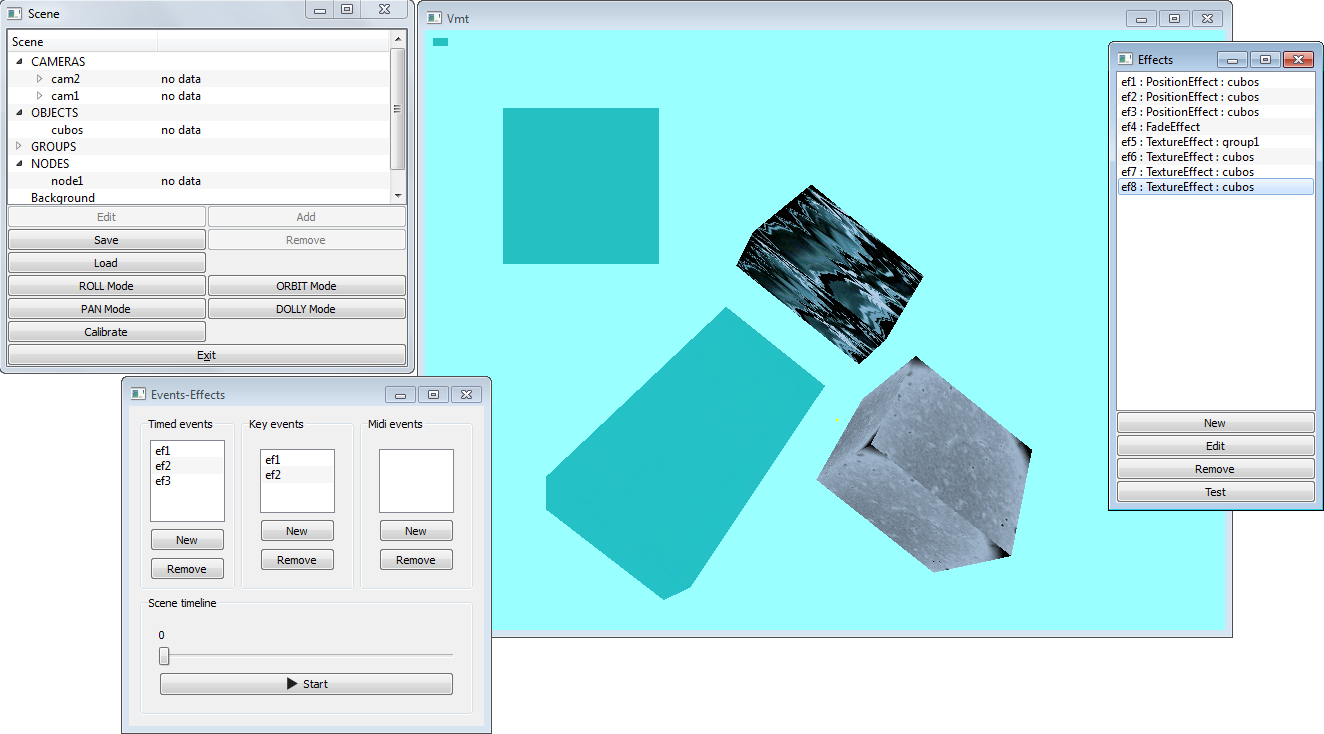
\includegraphics[width=0.7\textwidth]{./Cap5_vmt/vmt_todo.png}
  \caption{Vista general de la interfaz de usuario de VMT}
  \label{fig:VMT-MainWindow}
\end{figure}

Al inicio se cuenta con una vista gráfica de la escena desde el punto de vista de la cámara activa, una vista de los objetos contenidos en la escena, la lista de definición de efectos y una línea de tiempo con las listas de efectos por tiempo, por evento y MIDI.
En la ventana de escena se manejan los objetos bidimensionales y tridimensionales, cámaras, luces, capas y los nodos distribuidos del show. También es desde donde se ejecuta la calibración de las cámaras-proyectores. Para la visualización de la escena se ofrecen diferentes modos de cámara para girar u orbitar alrededor del centro, o moverse en cada uno de los ejes.

\begin{figure}[H]
  \centering
    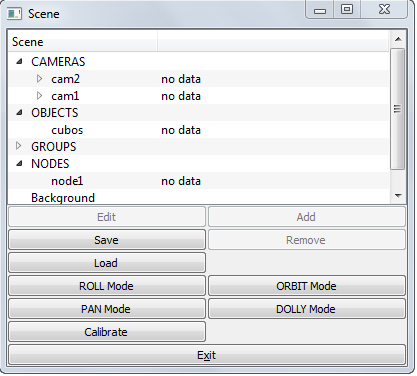
\includegraphics[width=0.5\textwidth]{./Cap5_vmt/vmt_scene.png}
  \caption{Ventana para manejar la escena}
  \label{fig:VMT-SceneWindow}
\end{figure}

\subsection{Cámaras, Capas y Quads}
Las cámaras tienen todas las propiedades usuales que se pueden encontrar en paquetes de software de animación tridimensional como ser Posición, Eye, Up, FOV (Field of View), Aspecto, Near, Far, etc.

\begin{figure}[H]
  \centering
    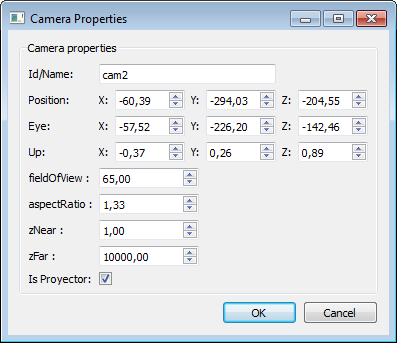
\includegraphics[width=0.5\textwidth]{./Cap5_vmt/vmt_cameraProperties.png}
  \caption{Dialogo de propiedades de cámara}
  \label{fig:VMT-CameraProperties}
\end{figure}

Se han modelado los proyectores como cámaras con marcas especiales, por lo cual a cada cámara se le puede indicar además si de lo que se trata en realidad es de un proyector. Esto permite contar tanto con cámaras para las cuales lo que veamos será lo que efectivamente saldrá proyectado, como también poder tener cámaras sin proyector asociado que nos permiten tener una vista en perspectiva de la escena para por ejemplo, experimentar como se vería el show desde el punto de referencia de un cierto observador.
Existen también acciones para seleccionar los tipos de movimiento de la cámara activa. Estos son:
Roll: posición y punto de vista fijos. Se rota alrededor del eje formado por ellos.
Orbit: distancia al punto de vista fijo. Se orbita a dicha distancia alrededor del punto de vista.
Dolly: punto y la dirección de vista fijos. Se mueve la posición de la cámara acercándose y alejándose del objetivo.
Pan: distancia al plano de la imagen fija. Se mueve cualquier dirección pero en plano paralelo al de la dirección.

\begin{figure}[H]
  \centering
    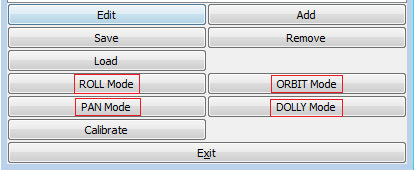
\includegraphics[width=0.5\textwidth]{./Cap5_vmt/vmt_SceneBotonera.png}
  \caption{Acciones para seleccionar modo de movimiento de la cámara activa}
  \label{fig:VMT-CameraActions}
\end{figure}

Una vez activado el modo de la cámara, manteniendo presionado el botón izquierdo del ratón al moverlo se mueve la cámara acorde al modo seleccionado.
Cada cámara es a su vez un contenedor de capas o layers. Su propósito es manejar todo lo relacionado al mapeo sobre estructuras bidimensionales, y por ello son los contendores de quads bidimensionales sobre los cuales se pueden realizar todas las operaciones y efectos disponibles.

\begin{figure}[H]
  \centering
    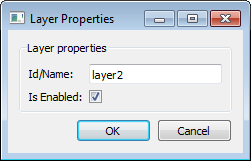
\includegraphics[width=0.5\textwidth]{./Cap5_vmt/vmt_layerProperties.png}
    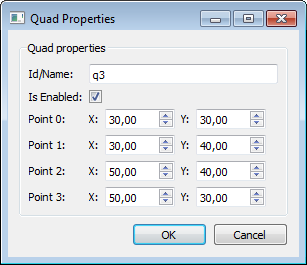
\includegraphics[width=0.5\textwidth]{./Cap5_vmt/vmt_quadProperties.png}
  \caption{Propiedades de los objetos Layer y Quad}
  \label{fig:VMT-LayerQuadProperties}
\end{figure}

Tanto el quad como la capa tienen propiedades editables en tiempo de edición o durante el show para mostrarse u ocultarse completamente. Si se oculta una capa, todos los quads contenidos en ella también serán ocultados. En caso de mostrarla, todos los quads visibles volverán a desplegarse.

\subsection{Objetos tridimensionales}

Se permite agregar objetos tridimensionales con formato de malla triangular del tipo 3DS [ref 3D-Studio File Format (.3ds) - Autodesk Ltd. - http://www.martinreddy.net/gfx/3d/3DS.spec ]. Para satisfacer los requerimientos actualmente definidos, solo fue necesario permitir la modificación del identificador y la posición de un objeto tridimensional.

\begin{figure}[H]
  \centering
    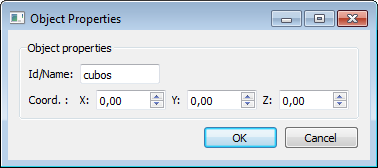
\includegraphics[width=0.5\textwidth]{./Cap5_vmt/vmt_objectProperties.png}
  \caption{Dialogo de propiedades de objeto tridimensional}
  \label{fig:VMT-ObjectProperties}
\end{figure}

\subsection{Efectos}

Es mediante un efecto que se declara lo que se hace o modifica en la escena, como y a que objetos. Se proveen ventanas flotantes tanto para la definición de efectos como para la asociación con sus disparadores como ser un instante de tiempo, un evento de teclado o un evento MIDI.

Si un efecto es definido para ser desplegado en un instante dado este se podrá visualizar cuando la línea de tiempo pase por ese instante. En caso de ser definido por evento este será visualizado cada vez que el evento asociado suceda, sea un evento de teclado o MIDI.
Los tipos de efectos posibles son de posición, degradé de color y mapeo de texturas.
Los efectos de posición son aplicables a objetos tridimensionales solamente, y lo que permiten es animar el objeto moviéndolo de una posición inicial a una final. Es posible definir una demora en la ejecución del efecto comenzando en el instante en el que debería ser mostrado (al pasar la línea de tiempo por el instante definido si es un efecto asociado a tiempo o al reconocerse el código de evento del efecto si es lanzado por eventos).

Figura: Dialogo de definición de efecto de tipo posición.

Los efectos de degradé solo son aplicables a grupos de quads y lo que permiten es pintar todos los quads del grupo de un color inicial e ir pasando por toda la gama de colores intermedios hasta llegar al color final. Para la selección de colores se utiliza un dialogo nativo para ese propósito. También es posible definir la duración del efecto.

Figura: Dialogo de definición de efecto de tipo degradé o fade.

Los efectos de tipo textura son aplicables tanto a grupos de quads como a objetos tridimensionales. Se pueden definir texturas de tipo Imagen o Video. En ambos casos es necesario proporcionar el camino al archivo multimedia correspondiente. Para el caso especifico de un efecto de textura asociado a un objeto tridimensional, es necesario proporcionar además la cara o conjunto de caras (lista de selección de faces) sobre los cuales se va a mapear el efecto de tipo textura definido.

Figura: Dialogo de definición de efecto de tipo textura (en este caso aplicada a un grupo).

Figura: Lista de efectos definidos en la escena.

Es posible testear el efecto que se está creando presionando el botón Test de la lista de efectos. Esto forzara la ejecución por una única vez del efecto seleccionado en la lista.

\subsection{Calibración}

El proceso de calibración en VMT se basa en posicionar cuatro puntos de la superficie donde se proyecta y cuatro puntos de la capa contenedora de quads para de esta forma calcular la matriz de transformación de la homografía que los hace corresponder.

Figura: Dialogo para configurar y ejecutar la calibración.

Al ingresar en el modo calibración se muestra en la pantalla de edición cuatro puntos azules de destino y cuatro puntos rojos de origen junto con el diálogo de configuración de la calibración.
El diálogo posee controles para posicionar cada uno de los ocho puntos mostrados en pantalla. Se deberán posicionar los cuatro puntos de origen en regiones significativas de la capa donde hayan vértices de quads preferiblemente alejados entre si. De esta forma se minimiza el error obtenido al calcular la matriz.
Los cuatro puntos de destino se deberán posicionar observando la proyección de estos sobre la superficie. Una vez los ocho puntos estén posicionados se podrá calcular y aplicar la nueva matriz de calibración presionando el botón OK.
Mediante el botón ReCalibrate se reestablece la calibración original, descartando los cambios realizados.

\subsection{Línea de tiempo}

Tanto para la fases de producción y revisión del evento como para la ejecución o reproducción del espectáculo en vivo, es necesario contar controles estándares para el manejo de la línea de tiempo.

Figura: Diálogo con línea de tiempo y lista de efectos asociados a tiempo y eventos.

La aplicación provee una forma de iniciar el evento mediante la acción de Start. Se provee una vista gráfica representada con una barra deslizante y una vista numérica para reflejar el avance en el tiempo en relación a la duración total del evento. Utilizando la barra deslizante es posible navegar por la línea de tiempo e iniciarla visualización del evento desde un instante cualquiera. Esto último es muy útil para la fase de pre-producción del espectáculo en la cual es muy común que el usuario se quiera concentrar en una ventana de tiempo específica en la que se está trabajando.

Figura: Asociación de eventos a instante de tiempo, evento y MIDI.

Sobre la linea de tiempo se pueden observar las listas de eventos agrupados por tipo, pudiéndose asociar cualquiera de los eventos previamente definidos a un instante dado o a un código de evento a ser utilizado durante el espectáculo, ya sea de teclado o proveniente de dispositivos de entrada MIDI.

\subsection{Nodos remotos}

Para modelar la red de nodos esclavos de VMT en los cuales se conectaran proyectores remotos es preciso definir, para cada nodo, su IP y puerto donde estarán configurados y la cámara definida en la escena que representará al proyector asociado.
  
Figura: Lista de nodos y dialogo de propiedades de nodos.

Esta información es necesaria para establecer el canal de comunicación con el proceso remoto y deducir que información se enviara al nodo en base a su cámara asociada. Recordar que las capas o layers están asociadas a una y solo una cámara, por lo cual si un efecto esta aplicado sobre un quad o grupo de quads, el mismo deberá ser propagado al nodo cuya cámara sea la que los contiene. En cuanto a los efectos aplicados sobre objetos tridimensionales, estos serán enviados a todos los nodos ya que todas las cámaras de todos los nodos tienen visibilidad de la escena tridimensional, aunque esta sea desde perspectivas diferentes.

\subsection{Escena en XML}
Se permite almacenar en archivos XML estándar una representación de lo que se ha definido en la escena. Para la búsqueda de los archivos XML se utilizan diálogos nativos para este propósito.

Figura XML save and load

\section{Decisiones de implementación}
Para la implementación del módulo de interfaz gráfica se siguió el patrón Model-View-Controller. Para cada ventana se generaron modelos que manejan los datos relevantes a cada una, impactando en el modelo general de la aplicación en caso de ser necesario.
Se utilizó Qt Framework [Qt - framework multiplataforma para la creación de aplicaciones e interfaces de usuario con APIs para C++. http://qt.nokia.com/products/] como biblioteca de base para la creación de las ventanas, sus controles gráficos y manejo de la comunicación que ocurre entre ventanas y con los modelos de VMT. También se hizo uso de la funcionalidad para internacionalización de las interfaces gráficas, las que por el momento están tomando valores por defecto en idioma Inglés. Es multiplataforma por lo que puede ser utilizado en varios de los sistemas operativos de computadores de escritorio mas populares como ser Linux, Mac OS y Windows. Esto último es un requerimiento no funcional del proyecto que fue tenido en cuenta al decidir incorporar a la aplicación bibliotecas o marcos de trabajo para su desarrollo.
